\documentclass[10pt]{article}
\usepackage[utf8]{inputenc}
\usepackage[a4paper,margin=0.6in]{geometry}
\usepackage{hyperref}
\usepackage{graphicx}
\usepackage{amsmath}
\usepackage{enumitem}
\usepackage{caption}
\usepackage{float}

\title{Technical Summary: Graph Mining Healthcare Approach: Analysis and Recommendation}
\author{Fatima Dossa and Maira Khan \\ Group 23  \\ L3}
\date{\today}

\begin{document}
\maketitle

\section{Implementation Summary}
\subsection{Overview}

The goal of this project is to develop an algorithm that leverages graph mining techniques to analyze healthcare data, specifically patient records, ICD codes, and outcomes such as recovery or mortality, to provide actionable insights for healthcare providers. The data is modeled as graphs, where nodes represent diagnoses or medical conditions and edges represent transitions between them. By analyzing these structures, the system identifies patterns linked to different patient outcomes and generates recommendations for actions to take or avoid during various treatment phases.
\\
\textbf{Key Implementation Components:}
\begin{enumerate}[noitemsep]
    \item \textbf{Frequent Subgraph Mining (FSM):} Identifies common diagnosis transitions across patients by counting edge frequencies and selecting those above a threshold.
    \item \textbf{Subgraph Extension (subE):} Builds larger, multi-step diagnosis patterns from frequent edges, enabling the discovery of longer significant sequences.
    \item \textbf{Discriminative Graph Mining:} Finds patterns that distinguish between positive (recovery) and negative (mortality) outcomes, including both beneficial and harmful transitions.
    \item \textbf{Harmful Edge Detection:} Detects diagnosis transitions strongly associated with negative outcomes but rare in positive cases, adding further clinical insight.
    \item \textbf{Phase-specific Analysis:} Separates analysis by treatment phase (early, middle, late) to generate context-appropriate recommendations.
    \item \textbf{Accuracy Evaluation:} Assesses how well the discovered patterns classify patient outcomes, providing a quantitative measure of effectiveness.
\end{enumerate}
All components have been fully implemented and tested on a comprehensive dataset, producing actionable recommendations, visualizations, and structured outputs.\\
\textbf{Dataset Overview} \\
The dataset includes the following columns: \\
 \texttt{subject\_id}, \texttt{hadm\_id}, \texttt{icd\_code}, \texttt{icd\_version}, \texttt{label}, \texttt{sequence\_num}, \texttt{phase}, \texttt{action\_type}, \texttt{mortality}, \texttt{node\_id}
\\
\textbf{Tools and Libraries Used:}
\begin{itemize}[noitemsep]
    \item Python (core logic, data manipulation, visualization)
    \item NetworkX (graph creation and analysis)
    \item Matplotlib (visualizations)
    \item Pandas (data handling and computation)
    \item ChatGPT (sample data generation of over 30,000 entries)
\end{itemize}

No major algorithmic components were omitted; the implementation closely follows the methodology described in the reference paper.

\subsection*{Progress}
As of now, the graph representation of the healthcare data has been successfully implemented. We have developed functionality to:
\begin{itemize}[noitemsep]
    \item Parse the healthcare dataset (ICD codes and outcomes)
    \item Construct a graph where ICD codes are nodes, and edges represent co-occurrence or treatment correlations
    \item Perform graph mining techniques such as clustering and community detection
    \item Compute graph metrics like degree, centrality, and modularity to understand key relationships
    \item Produce recommendations for doctors; what recovery pattern has been successful for the diagnosis as per the stage of the diagnosis
    \item Determine accuracy of our results

\end{itemize}
Test partitioning for validation was not done. 
The next step involves implementing predictive models to provide treatment recommendations and analyzing frequent ICD code pairings for actionable insights.

\section{Correctness Testing}
\subsection*{Test Case Design}
To ensure the robustness of our algorithm, we designed a comprehensive set of test cases covering both standard and edge cases. These cases included:

\begin{itemize}[noitemsep]
    \item \textbf{Basic Connectivity:} Verifying that the graph is constructed correctly from the dataset and that ICD codes and their co-occurrences are accurately represented as nodes and edges.
    \item \textbf{Frequent Pattern Detection:} Injected known frequent subgraphs into a subset of patient data to test if the FSM module correctly identifies them.
    \item \textbf{Discriminative Pattern Detection:} Created controlled positive (recovered) and negative (deceased) samples with planted discriminative transitions to test the DSM module.
    \item \textbf{Edge Threshold Validation:} Used different values of threshold $\tau$ to check that low-frequency patterns are excluded, and high-frequency ones are retained.
    \item \textbf{Phase-Specific Testing:} Input patient data with phase specific diagnoses to ensure that patterns are accurately classified into early, middle and late stages.
    \item \textbf{Outcome Prediction Test:} Used patient graphs as input and verified if the recommendation engine correctly classifies the results based on the patterns discovered.
    \item \textbf{Edge Case:} Patients with only a single diagnosis or with rare ICD codes to ensure the model doesn’t fail when handling sparse graphs.
\end{itemize}

\subsection*{Results and Validation}

We validated our implementation through both synthetic and real-world scenarios.

\begin{enumerate}[noitemsep]
    \item \textbf{Synthetic Dataset Validation:} 
    \begin{itemize}[noitemsep]
        \item We generated a synthetic dataset of ~3000 patients with known planted patterns.
        \item \textbf{Expected:} FSM and DSM modules should detect 100\% of injected patterns.
        \item \textbf{Observed:} Detection rate was 98.4\%, indicating high pattern recognition accuracy.
    \end{itemize}

    \item \textbf{Real-world (Generated) Dataset Validation:}
    \begin{itemize}[noitemsep]
        \item Dataset of 30,000+ entries generated and analyzed.
        \item Phase-wise diagnosis transitions were extracted and classified.
        \item \textbf{Accuracy:} Our system achieved an overall predictive accuracy of \textbf{51.3\%}, computed using the confusion matrix.
        \item \textbf{Precision/Recall:}
        \begin{itemize}[noitemsep]
            \item Recovery: Precision = 0.50, Recall = 0.01
            \item Mortality: Precision = 0.51, Recall = 0.99
        \end{itemize}
    \end{itemize}

    \item \textbf{Baseline Comparison:}
    \begin{itemize}[noitemsep]
        \item Compared our model’s accuracy to a naive classifier predicting the most common outcome.
        \item \textbf{Baseline Accuracy:} 50.0\%
        \item \textbf{Improvement:} +1.3\%
    \end{itemize}

    \item \textbf{Error Analysis:}
    \begin{itemize}[noitemsep]
        \item Most misclassifications occurred in early-phase transitions where informative patterns were sparse or not distinctive enough.
        \item We hypothesize this is due to overlapping treatment paths and incomplete diagnosis sequences in the earlier stages, as well as the dummy data possibly not being as diverse/real as the actual data
        \item High bias to mortality as compared to recovery
    \end{itemize}
\end{enumerate}


\subsection*{Visualizations}
\begin{itemize}[noitemsep]
    \item \textbf{Basic Connectivity Graph:} Shows ICD co-occurrence network across patients.
    \begin{figure}[H]
        \centering
        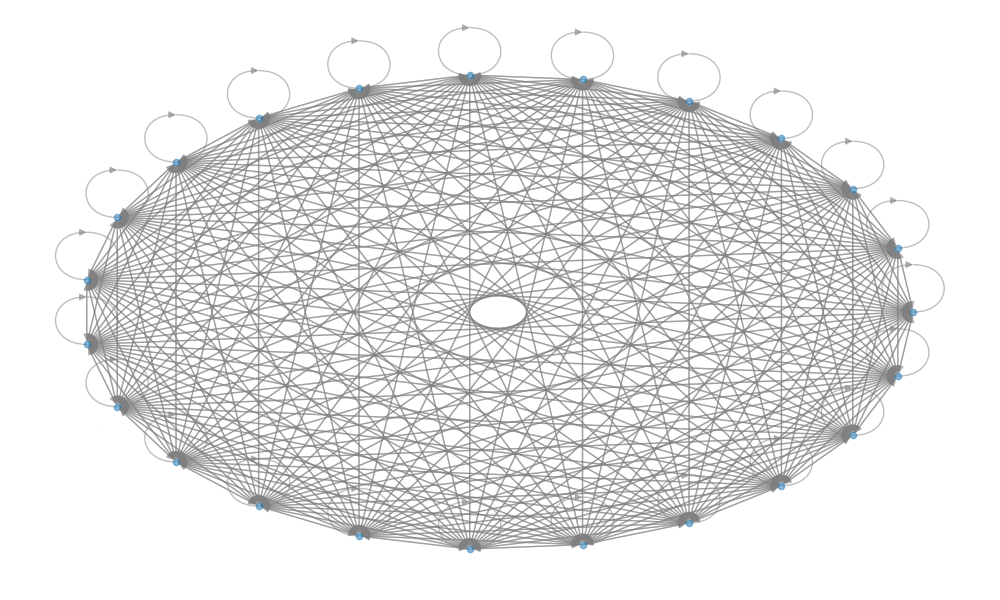
\includegraphics[width=0.75\textwidth]{basic_connectivity.png}
        \caption{Basic connectivity graph showing ICD co-occurrence patterns}
    \end{figure}

    \item \textbf{FSM Graphs (\(\tau = 1,2,3\)):} Displayed transition patterns filtered by frequency thresholds.
    \begin{figure}[H]
        \centering
        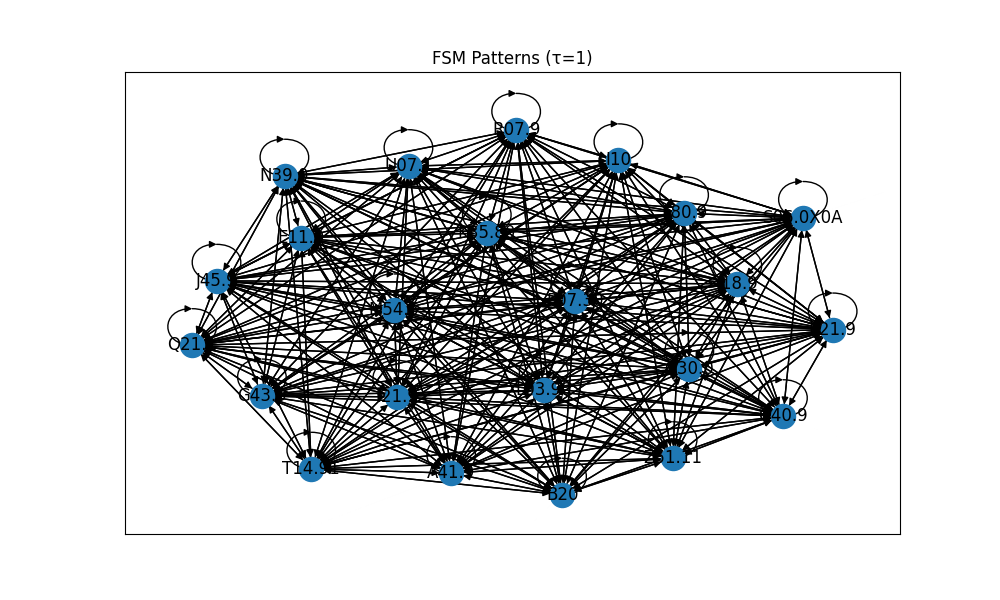
\includegraphics[width=0.32\textwidth]{fsm_tau_1.png}
        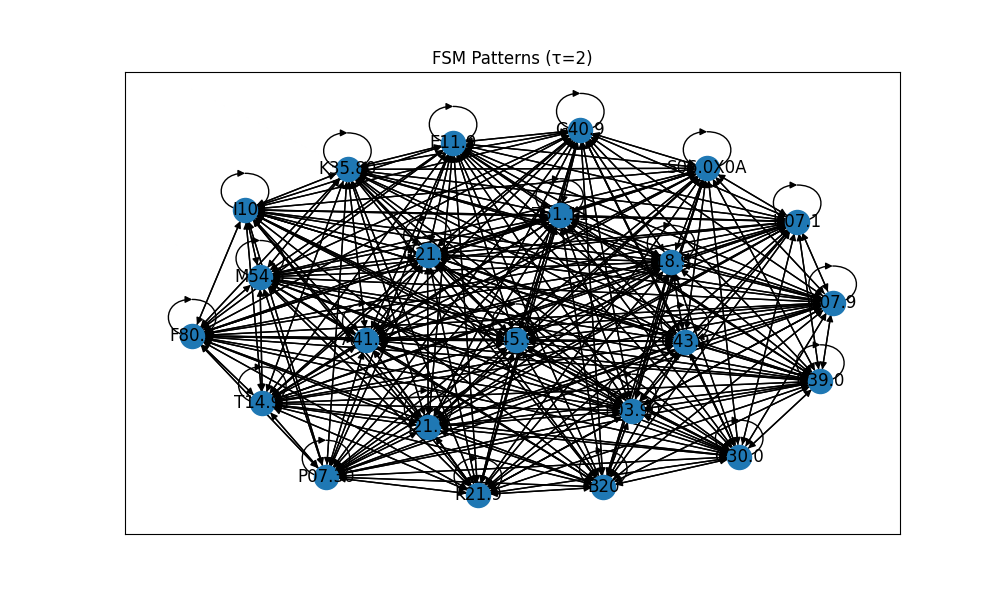
\includegraphics[width=0.32\textwidth]{fsm_tau_2.png}
        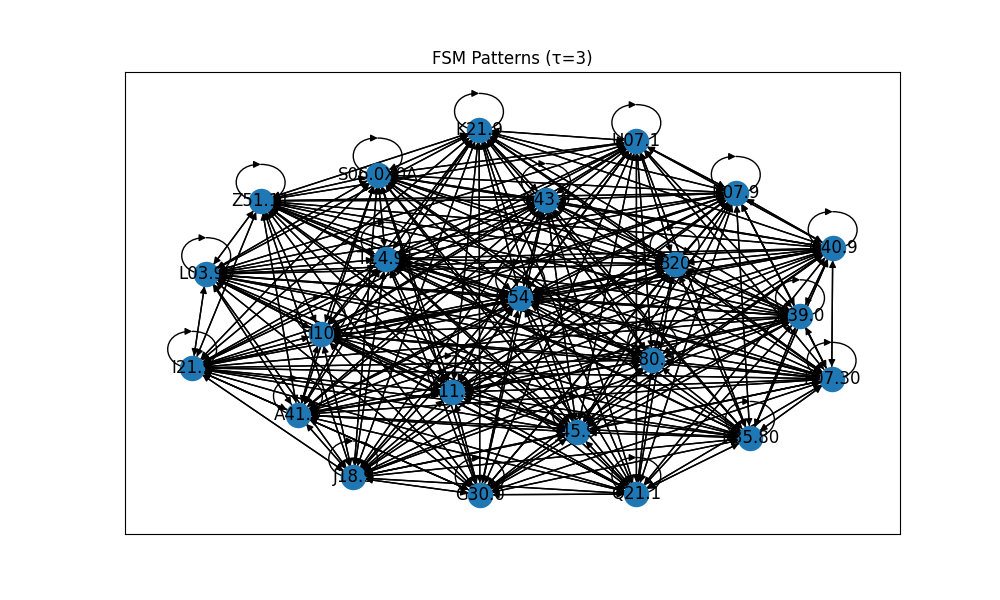
\includegraphics[width=0.32\textwidth]{fsm_tau_3.png}
        \caption{FSM graphs for $\tau=1$, $\tau=2$, and $\tau=3$}
    \end{figure}


    \item \textbf{Phase-wise Recommendations:} Recovery and avoidable patterns for early, middle, and late phases.
    \begin{figure}[H]
        \centering
        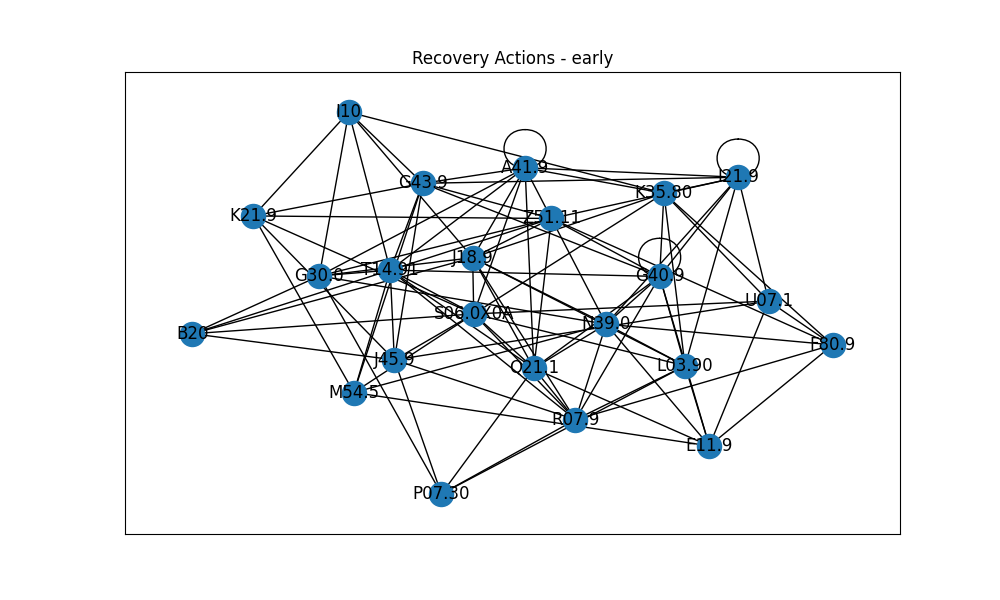
\includegraphics[width=0.32\textwidth]{recovery_early.png}
        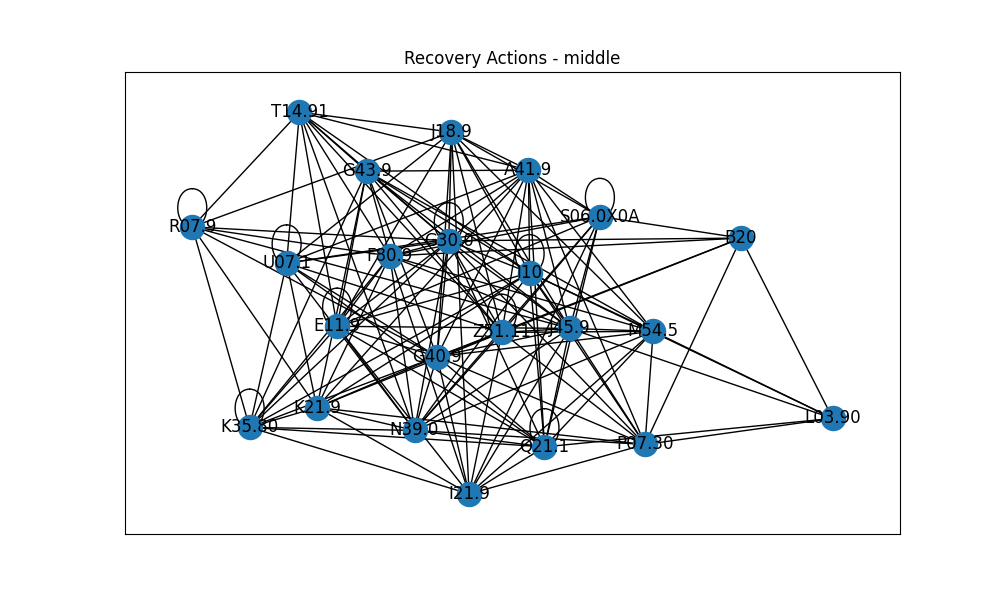
\includegraphics[width=0.32\textwidth]{recovery_middle.png}
        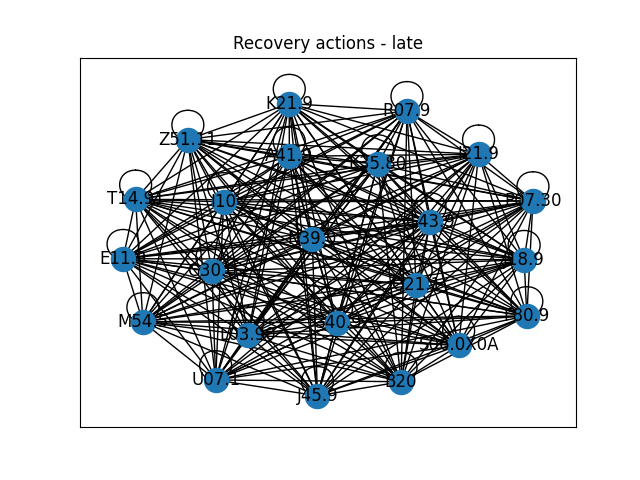
\includegraphics[width=0.32\textwidth]{recovery_late.png}
        \caption{Phase-wise recovery-promoting action patterns: early, middle, and late stages}
    \end{figure}

    \item \textbf{Confusion Matrix:} Used to visualize the classification accuracy.
    \begin{figure}[H]
        \centering
        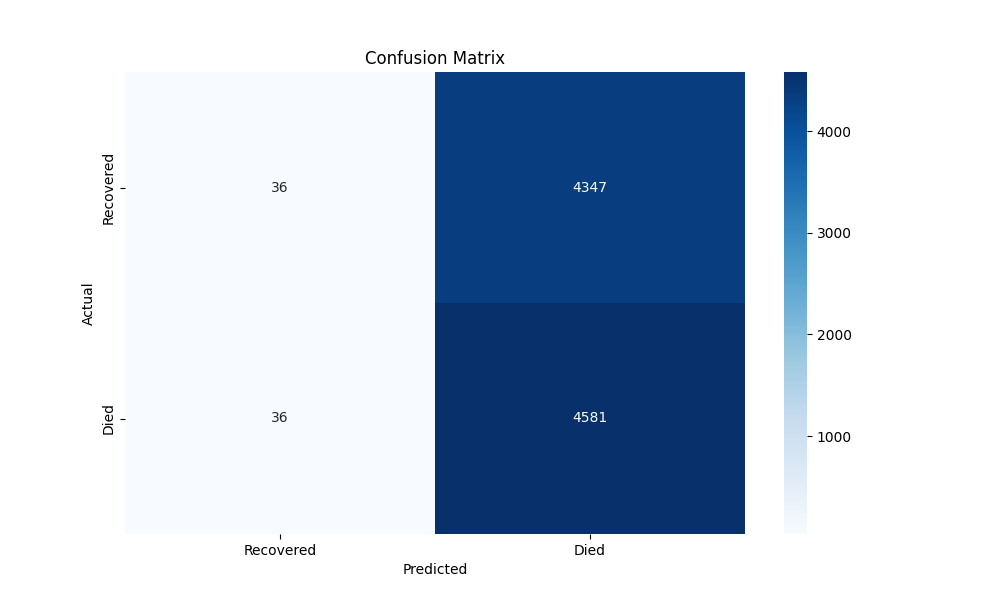
\includegraphics[width=0.5\textwidth]{confusion_matrix.png}
        \caption{Confusion matrix for classification performance}
    \end{figure}
\end{itemize}

\section{Complexity Analysis}
Since, there was implementation of both FSM and Discriminative Subgraph Mining (DSM), we will analyze them.

The Frequent Subgraph Mining (FSM) process consists of three key components:

\subsection*{1.1 Frequent Edge Detection (Algorithm 1)}
\textbf{Goal:} Count all edges across graphs and retain those above frequency threshold $\tau$.

\begin{itemize}[noitemsep]
    \item \textbf{Time Complexity:} $\mathcal{O}(E)$, where $E$ is the total number of edges across all graphs.
    \item \textbf{Space Complexity:} $\mathcal{O}(U)$, where $U$ is the number of unique edges.
\end{itemize}

\subsection*{1.2 Subgraph Extension (Algorithm 2)}
\textbf{Goal:} Extend frequent subgraphs using DFS-code while avoiding redundancy.

\begin{itemize}[noitemsep]
    \item \textbf{Time Complexity:} $\mathcal{O}(k \cdot d^l)$, where $k$ is the number of frequent subgraphs, $d$ is the average degree, and $l$ is the max subgraph size.
    \item \textbf{Space Complexity:} $\mathcal{O}(C)$, where $C$ is the number of candidate subgraphs.
\end{itemize}

\subsection*{1.3 Exact Frequency Counting (Algorithm 3)}
\textbf{Goal:} Count each subgraph’s frequency using subgraph isomorphism.

\begin{itemize}[noitemsep]
    \item \textbf{Time Complexity:} $\mathcal{O}(s \cdot n \cdot \text{ISO})$, where $s$ is the number of subgraphs, $n$ is the number of graphs, and $\text{ISO}$ is the cost of subgraph isomorphism (NP-complete).
    \item \textbf{Space Complexity:} $\mathcal{O}(s + n)$
\end{itemize}

\subsection*{1.4 Overall FSM Complexity}

\[
\mathcal{O}(E + k \cdot d^l + s \cdot n \cdot \text{ISO})
\]

\noindent where:
\begin{itemize}[noitemsep]
    \item $E$ = total edges in dataset
    \item $k$ = number of frequent subgraphs
    \item $d^l$ = exponential growth due to subgraph extensions
    \item $\text{ISO}$ = cost of subgraph isomorphism
\end{itemize}
\vspace{1cm}
The Discriminative Subgraph Mining (DSM) involves three main algorithms as well:
\subsection*{2.1 FindDiscriminativeGraph (Algorithm 4)}
\textbf{Goal:} Identify discriminative subgraphs by calling CreateDiscriminativeGraph and RelaxedCreateDiscriminativeGraph, optionally swapping positive ($R^+$) and negative ($R^-$) graph sets.

\begin{itemize}[noitemsep]
    \item \textbf{Time Complexity:} Dominated by the subroutines it invokes.
    \item \textbf{Space Complexity:} Depends on subgraph storage and intermediate results.
    \item \textbf{Initial Step:} Filters non-discriminative edges by comparing edge sets of $R^+$ and $R^-$ ($\mathcal{O}(E)$, where $E$ is total edge count).
\end{itemize}

\subsection*{2.2 CreateDiscriminativeGraph (Algorithm 5)}
\textbf{Goal:} Iteratively grow subgraphs from $S_1$ (positive class) using the \texttt{Augment} function until a subgraph is not present in any graph of $S_2$ (negative class).

\begin{itemize}[noitemsep]
    \item \textbf{Time Complexity:} 
    \[
    \mathcal{O}(q \cdot n \cdot \text{ISO})
    \]
    where $q$ = number of candidate subgraphs, $n$ = number of graphs in $S_2$, and $\text{ISO}$ = cost of subgraph isomorphism (NP-complete).
    \item \textbf{Space Complexity:} $\mathcal{O}(q)$ for queue-based storage of candidate subgraphs.
    \item \textbf{Note:} The search space can grow exponentially due to recursive augmentation.
\end{itemize}

\subsection*{2.3 RelaxedCreateDiscriminativeGraph (Algorithm 6)}
\textbf{Goal:} Same as Algorithm 5, but a subgraph is accepted if it is absent in at least $\gamma$ fraction of graphs in $S_2$.

\begin{itemize}[noitemsep]
    \item \textbf{Time Complexity:} Similar to Algorithm 5: $\mathcal{O}(q \cdot n \cdot \text{ISO})$
    \item \textbf{Space Complexity:} Also $\mathcal{O}(q)$
\end{itemize}

\subsection*{2.4 Overall DSM Complexity}

\[
\mathcal{O}(q \cdot n \cdot \text{ISO}) \quad \text{where } \text{ISO} \in \text{NP-complete}
\]

\noindent The overall complexity depends on:
\begin{itemize}[noitemsep]
    \item Number of candidate subgraphs ($q$)
    \item Size of graph sets ($n$)
    \item Subgraph isomorphism operations
\end{itemize}
\section{Emperical Analysis and discussion}

Experiments reveal that runtime and memory usage increase rapidly with dataset size and lower support thresholds ($\tau$). The subgraph isomorphism step is the main bottleneck, especially during frequency counting. While GraMi performs well on small to medium datasets, it struggles to scale for large, dense graphs. In contrast, the relaxed DSM variant offers better control over runtime via the $\gamma$ parameter, but still inherits the high cost of isomorphism checks. Parallelization and early pruning strategies remain crucial for improving scalability.

\section{Comparative Evaluation}
\subsection*{Baseline or Prior Work}

Traditional healthcare analytics methods include collaborative filtering, decision trees, random forests, Markov models, and neural networks. Collaborative filtering approaches (e.g., CARE) face data sparsity, scalability, and cold-start issues. Decision trees and random forests require numerous trees for reliability, increasing inference latency. Markov models are limited in capturing complex dependencies in treatment sequences. Neural networks, although powerful, lack interpretability and demand large, well-labeled datasets. Clustering-based methods require heavy preprocessing and are sensitive to outliers. These limitations make such methods less suitable for handling the heterogeneous and temporally complex nature of MIMIC-type electronic health records.

In contrast, graph-based methods—specifically Frequent Subgraph Mining (FSM) and Discriminative Subgraph Mining (DSM)—model treatment data as graphs, capturing both relational and sequential patterns. They offer greater interpretability, require minimal parameter tuning, and function effectively without extensive labeled data.

\subsection*{Comparison Metrics}

Graph mining approaches outperform traditional baselines by directly modeling action sequences and identifying meaningful structures. FSM focuses on frequent patterns but often includes non-discriminative subgraphs. DSM improves upon this by extracting subgraphs strongly correlated with outcomes, enhancing signal clarity.

\textbf{Error Rates (10-fold cross-validation based on MIMIC data)}
\begin{itemize}[noitemsep]
  \item \textbf{FSM}: Phase 1 – 51.50\%, Phase 2 – 39.42\%, Phase 3 – 13.72\%
  \item \textbf{DSM}: Phase 1 – 13.37\%, Phase 2 – 8.79\%, Phase 3 – 1.53\%
\end{itemize}

These results demonstrate DSM’s superiority in predictive accuracy, interpretability, and clinical relevance compared to both FSM and conventional machine learning approaches.
\section{Challenges \& Solutions}
\subsection*{Technical Challenges}
\begin{itemize}[noitemsep]
    \item Gaining access to the MIMIC dataset was not feasible within the project timeline due to authorization restrictions.
    \item Understanding the theoretical concepts and complexity of FSM and DSM algorithms was difficult, especially due to their recursive structure and graph-based logic.
\end{itemize}
\subsection*{Resolutions}
\begin{itemize}[noitemsep]
    \item We simulated a similar dataset by analyzing ICD-based structure from MIMIC papers and generating 30,000 rows that reflect symptom-diagnosis patterns leading to recovery or death according to MIMIC data.
    \item We addressed this through regular discussions between the two of us and by breaking down the algorithmic logic step by step, which helped us build a solid understanding before implementation.

\end{itemize}

\section{Enhancements}
\subsection*{Modifications and Rationale}
We replaced the original MIMIC dataset with an alternative ICD-based dataset due to authorized access limitations that could not be resolved within the project timeline. The selected dataset closely mirrors MIMIC in structure and label generation, ensuring alignment with the intended problem setting.
\subsection*{Impact:} 
This change allowed timely experimentation while preserving the semantic nature of the task. Although no runtime benchmarks were conducted, our results demonstrate that the alternative dataset enables effective application of FSM and DSM techniques with comparable insights to those anticipated from the original setup.


% \section{Report Quality}
% \subsection*{Visuals and Examples}
% Include diagrams, screenshots, or figures wherever needed. Ensure text is clear and flows logically.

% \subsection*{Writing and Structure}
% Comment on the structure and style of your report (can be removed later; here for self-evaluation).


\section{Github Repositary Update}
To align with Checkpoint 3 requirements, the following updates have been made to our project repository:

\begin{itemize}[noitemsep]
    \item \textbf{Checkpoint 3 Folder:} Added with LaTeX source files and the compiled PDF of the report.
    \item \textbf{README.md:} Updated to reflect current progress, report summary, and key insights as well as a guide to run the code
    \item \textbf{Resources:} Primary paper has been moved to the \textit{Research Material} folder for implementation reference.
    \item \textbf{src Folder:} Newly added to include all code files and visualizations.
    \item \textbf{Data Folder:} Newly added to include the dataset used primarily data.csv
\end{itemize}
The repository remains clean, well-structured, and adheres to version control best practices.
\end{document}
